\documentclass[11pt,a4paper,titlepage]{article}
\usepackage[utf8]{inputenc}
\usepackage{amsmath}
\usepackage{amsfonts}
\usepackage{amssymb}

\usepackage{tikz}
\usetikzlibrary{calc,patterns,angles,quotes,shapes.geometric, arrows}
\tikzstyle{train} = [rectangle, rounded corners, minimum width=2.2cm, minimum height=1cm,text centered, draw=black, fill=red!30]
\tikzstyle{test} = [rectangle, rounded corners, minimum width=2.2cm, minimum height=1cm,text centered, draw=black, fill=green!30]
\tikzstyle{data} = [rectangle, rounded corners, minimum width=11.8cm, minimum height=1cm,text centered, draw=black, fill=gray!30]
\tikzstyle{MSE} = [rectangle, rounded corners, minimum width=1.4cm, minimum height=1cm,text centered, draw=black, fill=orange!30]
\tikzstyle{arrow} = [thick,->,>=stealth]

\usepackage{float}
%\usepackage{mathtools}
\usepackage{bm}
\usepackage[margin=1in]{geometry}

\title{Project 1 in FYS-STK4155}
\author{Adrian Martinsen Kleven & Simon Elias Schrader }
\date{Autumn 2020}
\usepackage{hyperref}

\usepackage{natbib}
\usepackage{graphicx}
\graphicspath{{../figures/presentable_data/}} %Setting the graphicspath

\begin{document}
%\maketitle
\tableofcontents
\listoffigures
\listoftables

\clearpage
\section{Abstract}
In this project, we use some good methods and some shitty methods to test how well a polynomial can interpolate a superfancy exponential function (protip: It can't) . Then we use the same approaches to see how well random geographic data can be approximated. We expect this to look horrible. We're sorry for abusing math in that way. We shall contemplate Seppuku.

\begin{figure}[H]
\centering

\includegraphics[scale=1.7]{universe}
\caption{Some random picture.}
\label{fig:universe}
\end{figure}
\section{Introduction}
\section{Methods}
\subsection{Linear Regression}
The aim of Linear Regression is to find the conditional distribution $p(y|\bm{x})$ for y given $\bm{x}$. In Linear Regression, a linear functional dependence is assumed, and the aim is hence to create a linear function that fits a set of $p$ predictor variables $\bm{x}$ to a target variable $\bm{y}$, where there are $n$ discrete observations for each of the $p$ predictor variables and the target variable. That is, the aim is to find a functional relationship of the form $f(\bm{x})=y$. \\
We assume hence that each target variable $y_i$ has a functional dependence of the predictor variables:
\begin{equation*}
y_i= \tilde{y}_i+\epsilon_i=\beta_0 + \beta_1x_{i0} + \beta_2x_{i1}+...+\beta_px_{i(p-1)} + \epsilon_i
\end{equation*}
As this is true for all y, this can be written in matrix form:
\begin{equation*}
\bm{y}= \bm{X\beta} + \bm{\epsilon}
\end{equation*}
where $\bm{y}$, and $\bm{\epsilon}$ are vectors of length n,  $\bm{\beta}$ is of length p and $\bm{X}$ is a matrix of size $n*p$. X is called the design matrix.
 We now want to find fitting parameters $\bm{\beta}$ that represent the best linear fit of y to the input data $\bm{x}$. Hence, we want the fit
 \begin{equation*}
 \bm{\tilde y}= \bm{X\beta}
 \end{equation*}
 to be as close to the target data $\bm{y}$ as possible.
  There are several approaches to define the best linear fit, and in this article, we looked at three different methods that define the best fit in a different way each. All methods have in common that they define a loss function, which describes the deviation from the fit to the real data, that needs to be minimized.
\subsubsection{Ordinary Least Squares Regression}
In Ordinary Least Square regression, the loss function is defined as the following:
\begin{equation*}
C(\bm{\beta})= \frac{1}{n}\sum_{i=0}^n\left( y_i-\tilde y_i \right)^2
=\frac{1}{n}(\bm{y}-\bm{\tilde y})(\bm{y}-\bm{\tilde y})^T=
\frac{1}{n}(\bm{y}-\bm{X\beta})(\bm{y}-\bm{X\beta})^T
\end{equation*}
The solution minimizing this problem is found by deriving $C(\bm{\beta})$ with regards to each $\beta_i$ and setting each derivative equal to zero. Doing this, we end up with the following equation (in matrix notation)
\begin{equation*}
\frac{\partial C(\bm{\beta})}{\partial\bm{\beta}}=0=\bm{X^T}(\bm{y}-\bm{X\beta})
\end{equation*}
which gives us
\begin{equation*}
\bm{\beta}=(\bm{X}^T\bm{X})^{-1}\bm{X}^T\bm{y}
\end{equation*}
which can be solved when $(\bm{X}^T\bm{X})$ is invertible. In the case of strongly correlated data and large matrices, There might be issues in inverting $(\bm{X}^T\bm{X})$ due to the matrix being singular. Also, for very large matrices, there might be issues caused by the fact that many mathematical operations can introduce a numerical error. Hence, an equivalent, but more stable way to implement the solution for $\bm{\beta}$ is to use Singular Value Decomposition (SVD). As every matrix has a SVD decomposition, we can write
\begin{equation}\label{SVD_OLS}
\begin{split}\bm{\beta} & =\left(\bm{X}^T\bm{X}\right)^{-1}\bm{X}^T\bm{y}\\
& = \left(\bm{V}\bm{D}^T\bm{U}^T\bm{U}\bm{D}\bm{V}^T\right)^{-1}\bm{V}\bm{D}^T\bm{U}^T\bm{y}\\
& = \left(\bm{V}\bm{D}^T\bm{I}_p\bm{D}\bm{V}^T\right)^{-1}\bm{V}\bm{D}^T\bm{U}^T\bm{y}\\
& = \left(\bm{V}\bm{D}^2\bm{V}^T\right)^{-1}\bm{V}\bm{D}^T\bm{U}^T\bm{y}\\
& = \bm{V}\bm{D}^{-2}\bm{V}^T\bm{V}\bm{D}^T\bm{U}^T\bm{y}\\
& = \bm{V}\bm{D}^{-1}\bm{U}^T\bm{y}\end{split}
\end{equation}.

Under the assumption that true data y is given as
\begin{equation*}
\bm{y}=f(\bm{x})+\bm{\epsilon}
\end{equation*}
where $\bm{\epsilon}$ follows a normal distribution $N(0,\sigma^2)$, information about the variance and the expectation value can be deduced. Assuming that $f(\bm{x})=\bm{X\beta}$, it can be shown that
\begin{equation*}
\mathbb{E}(y_i)=\bm{X_{i,*}\beta}
\end{equation*}

\begin{equation*}
Var(y_i)=\sigma^2
\end{equation*}

where $\bm{X_{i,*}}$ is the i-th row of the design matrix.

For $\beta$, it can be shown that
\begin{equation*}
\mathbb{E}(\bm{\beta})=\bm{\beta}
\end{equation*}
\begin{equation*}
Var(\bm{\beta})=\sigma^2(\bm{X}^T\bm{X})^{-1}
\end{equation*}
\subsubsection{Ridge Regression}
The above mentioned problems with OLS regression, namely those of correlated data and near singular matrices, can be amended by implementing ridge regression. This is done by introducing the regularization parameter $ \lambda$ in the cost function:
\begin{equation*}
    C(\boldsymbol{X},\boldsymbol{\beta})=\frac{1}{n}\left\{(\boldsymbol{y}-\boldsymbol{X}\boldsymbol{\beta})^T(\boldsymbol{y}-\boldsymbol{X}\boldsymbol{\beta})\right\}+\lambda\boldsymbol{\beta}^T\boldsymbol{\beta}
\end{equation*}
effectively imposing a penalty on the size of $\boldsymbol{\beta}$. This has the effect of decreasing the variance of the parameters $\beta$, and thereby reducing the impact of overfitting.\\The expression for the optimal value of $\boldsymbol{\beta}$ becomes

\begin{equation*}
    \boldsymbol{\beta}^{\mathrm{Ridge}} = \left(\boldsymbol{X}^T\boldsymbol{X}+\lambda\boldsymbol{I}\right)^{-1}\boldsymbol{X}^T\boldsymbol{y}.
\end{equation*}
Where as before the matrix $\boldsymbol{X}^T\boldsymbol{X}$ could have been singular, by adding a non- zero, positive value to the diagonal, the eigenvalues become positive definite ensuring that the matrix is invertible.
\paragraph*{Regularization parameter}
There are several factors that determine how different regularization parameters $\lambda$ will minimize the cost function. A dataset with a lot of noise will cause more overfitting at higher model complexities. We expect that increasing the noise parameter $\sigma$ in a model dataset will make models with a larger value of $\lambda$, perform better. We see an example of this in figure \ref{lambdatonoise}, where models with higher values of $\lambda$ give the smallest MSE with increasing noise.
\begin{figure}[H]
\centering

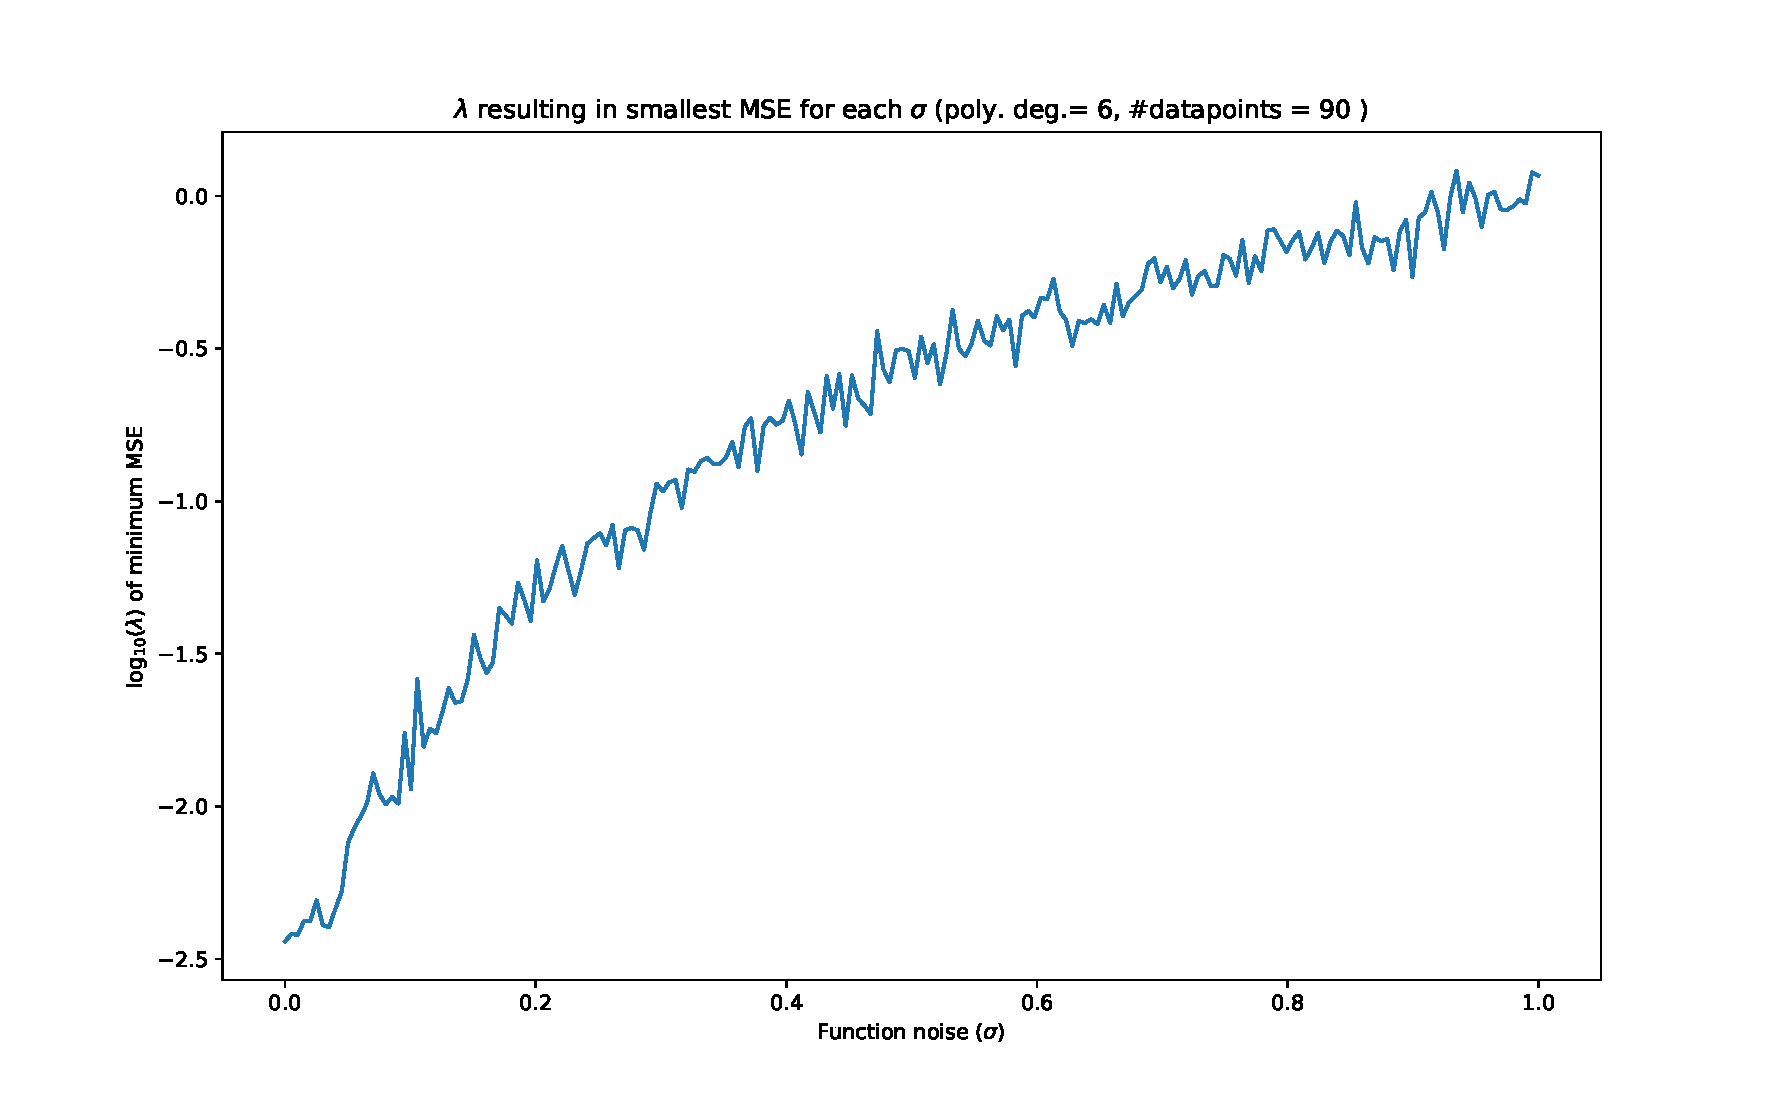
\includegraphics[trim=2cm 1.0cm 2cm 1.4cm, clip=true,scale = 0.5]{Smallest_MSE_lambda_over_noise.pdf}
\caption[Optimal regularization parameter to noise]{Performing Ridge regression on the Franke function \eqref{FrankeFunction}, with a normally distributed error term $\sigma\epsilon$.}\label{lambdatonoise}
\end{figure}
\subsubsection{LASSO Regression}
As with ridge, LASSO regression implements a new component to the cost function. Only, in this case the penalty is proportional to the L1- norm $\vert\vert \boldsymbol{\beta}\vert\vert$:
\begin{equation*}
    C(\boldsymbol{X},\boldsymbol{\beta})=\frac{1}{n}\left\{(\boldsymbol{y}-\boldsymbol{X}\boldsymbol{\beta})^T(\boldsymbol{y}-\boldsymbol{X}\boldsymbol{\beta})\right\}+\lambda\vert\vert \boldsymbol{\beta}\vert\vert.
\end{equation*}
One of the problems with ridge regression is that rather than eliminating covariant features, it will tend to shrink parameters, reducing their influence but not removing them. This is due to the behaviour of the squaring term in the L2- norm, which penalizes few large numbers more than many small numbers. For example, $\vert\vert[\beta_1,\beta_2]\vert\vert_2 \leq \vert\vert[\beta_1+\beta_2,0]\vert\vert_2$. Whereas in LASSO, the area of the L1- norm in the parameter space is more likely to intersect the least square loss function along the orthogonal axes in the paramater space, along which, at least one of the parameters are zero. This has a greater effect on eliminating features in a model, although which of two collinear parameters are eliminated is arbitrary.
\subsection{Resampling Methods and Data Splitting}
In order to get an approximate estimate of the quality of a fit, it is necessary that the fit is tested on a set that it has not been trained on. As the training set determines the parameters $\bm{\beta}$, we need a set from the same distribution as the training set, which is different from the training set. For that reason, the full data set of predictors and targets is split into a test set and a training set. The test usually contains $20-25\%$ of the full set, while the training set contains $75-80\%$. It is also possible to use a further validation set to do a final estimate using data that has never been "seen" by the programmer or the code, however, this was not implemented in this project.
\subsection{Bias-variance relationship}
In order to evaluate the quality of a fit, it is customary to evaluate the Mean Square Error (MSE) of the test data to the prediction. The Mean Square Error is defined as
\begin{equation*}
MSE(\bm{y},\bm{\tilde y})=n^{-1}\sum_i^N\left(y_i - \tilde y_i \right)^2=\mathbb{E}\left[(\bm{y}-\bm{\tilde y})^2  \right]
\end{equation*}
where the left formula is the within-sample mean square error.
The Mean Square Error can be decomposed into three parts: The unavoidable Error $\sigma^2$, the squared Bias (which is the deviation of the mean value of an estimator and the true value), and the Variance (which is a measure of the spread of the estimator). Hence
\begin{equation*}
MSE(\bm{y},\bm{\tilde y})=Bias[ \bm{\hat y}]^2 + Var[ \bm{\tilde y}]+\sigma^2= \left(f-\mathbb{E}(\tilde f)\right)^2 + \mathbb{E}\left(\left[\mathbb{E}\left[ \tilde f \right]-f\right)^2 \right]+\sigma^2
\end{equation*}
A proof of this decomposition can be found in the appendix.
In this article, we will however calculate the following values:
\begin{equation*}
Bias[\bm{\tilde y}]^2=n^{-1}\sum_i^N\left( y_i - avg( \bm{\tilde y})\right)^2
\end{equation*}
\begin{equation*}
Var[\bm{\tilde y}]^2=n^{-1}\sum_i^N\left(\tilde y_i - avg( \bm{\tilde y})\right)^2
\end{equation*}
This is because the true values $f_i$ are not known and impossible to obtain.\\
An important observation when fitting the data is that the Bias decreases as the model gets more complex, while the variance increases. When the Bias is large, important relations of the underlying data are not considered. When the Variance is high, small, unimportant features in the training set have too high of an impact. This is called overfitting. The aim is hence to find the model complexity that gives the lowest MSE. This is usually the case around the point where the Bias has the same magnitude as the Variance.
\subsubsection{Bootstrap method}
The Bootstrap method is a method that can be used to calculate statistical quantities. The main idea is the following: Let n be the size of the training set $Z=(z_1,z_2,...z_n)$, where each $z_i$ contains p predictors and one target value, that is $z_i=(x_{i,1},x_{i,2},...x_{i,p},y_i)$. Now, n data points $z_i$ are drawn randomly from Z with replacement. This is done $B$ times, creating $B$ new sets $Z'_j$. We can now create a fitting model for each of the sets  $Z'_j$. For each of these data sets $Z'_j$, we can now calculate any variable $\hat\theta_j$ given the data. Now, the distribution of $\hat\theta_j$ can be used to estimate the distribution of $\theta$ and get values of interest, such as the mean value or the variance. In this article, Bootstrap is used to get information about the test MSE, variance and bias in order to evaluate the quality of the fit. This is done by using the B bootstrap sets $Z'_j$ to calculate the fitting parameters $\beta$ and calculate B fits to the test set. $\tilde{Y_j}$. From these B fits, we can then approximate the test MSE, variance and bias.\\
TODO: Talk some more about the mathematical validity of Bootstrap.
\subsubsection{K-fold Cross validation}
K- fold Cross Validation is a useful technique for when you have a limited data set, and want to make sure that all features are captured in a training set. K- fold Cross Validation does this by partitioning the data set into $k$ so called folds, assigning $k-1$ folds as the training set and $1$ of the folds as the testing set. It does this $k$ times, making sure to utilize each fold as the testing set once. In this way, we end up generating $k$ different models, whose performance can be measured with respect to the testing fold or additionally, a separate testing set, withheld from the partitioning process.

\begin{figure}[H]
\centering
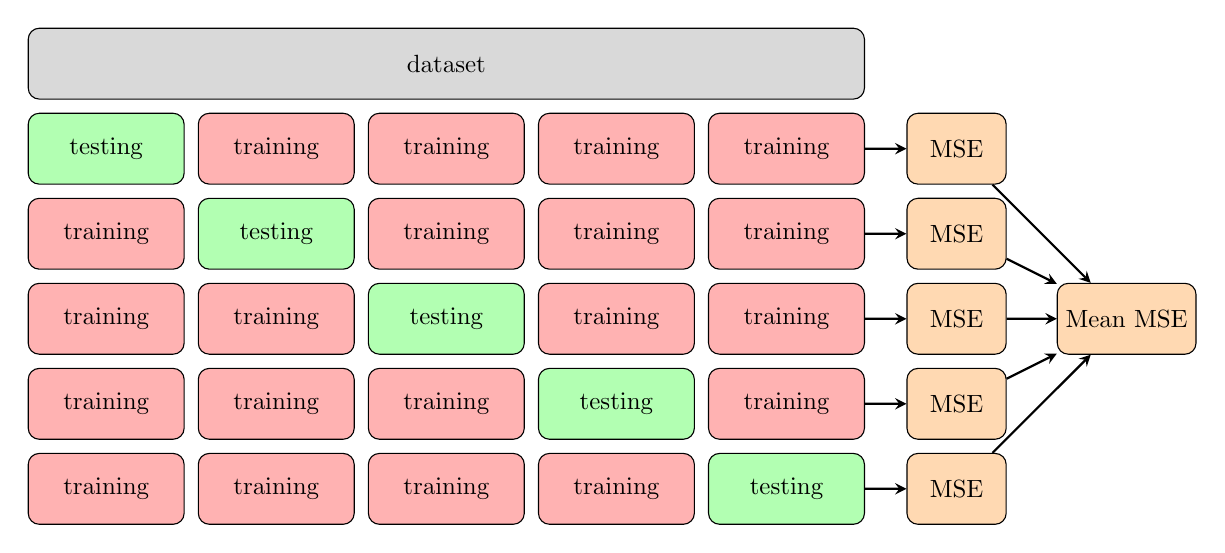
\begin{tikzpicture}[node distance=2.4cm,scale=0.9, every node/.style={scale=0.9}]

\node (data1)[data]{dataset};
\node (test1)[test,below of =data1,yshift =1.2cm,xshift=-4.8cm]{testing};
\node (train1) [train,right of=test1] {training};
\node (train2) [train,right of=train1] {training};
\node (train3) [train,right of=train2] {training};
\node (train4) [train,right of=train3] {training};
\node (MSE1) [MSE,right of=train4] {MSE};
\draw [arrow] (train4) -- (MSE1);

\node (test12)[train,below of =test1,yshift =1.2cm]{training};
\node (train12) [test,right of=test12] {testing};
\node (train22) [train,right of=train12] {training};
\node (train32) [train,right of=train22] {training};
\node (train42) [train,right of=train32] {training};
\node (MSE2) [MSE,right of=train42] {MSE};
\draw [arrow] (train42) -- (MSE2);

\node (test13)[train,below of =test12,yshift =1.2cm]{training};
\node (train13) [train,right of=test13] {training};
\node (train23) [test,right of=train13] {testing};
\node (train33) [train,right of=train23] {training};
\node (train43) [train,right of=train33] {training};
\node (MSE3) [MSE,right of=train43] {MSE};
\draw [arrow] (train43) -- (MSE3);

\node (test14)[train,below of =test13,yshift =1.2cm]{training};
\node (train14) [train,right of=test14] {training};
\node (train24) [train,right of=train14] {training};
\node (train34) [test,right of=train24] {testing};
\node (train44) [train,right of=train34] {training};
\node (MSE4) [MSE,right of=train44] {MSE};
\draw [arrow] (train44) -- (MSE4);

\node (test15)[train,below of =test14,yshift =1.2cm]{training};
\node (train15) [train,right of=test15] {training};
\node (train25) [train,right of=train15] {training};
\node (train35) [train,right of=train25] {training};
\node (train45) [test,right of=train35] {testing};
\node (MSE5) [MSE,right of=train45] {MSE};
\draw [arrow] (train45) -- (MSE5);

\node (MSEtot) [MSE,right of=MSE3] {Mean MSE};
\draw [arrow] (MSE1) -- (MSEtot);
\draw [arrow] (MSE2) -- (MSEtot);
\draw [arrow] (MSE3) -- (MSEtot);
\draw [arrow] (MSE4) -- (MSEtot);
\draw [arrow] (MSE5) -- (MSEtot);


\end{tikzpicture}
\caption[K-fold Cross Validation operation structure]{In this example, 5- fold Cross Validation is used on the entire dataset, with one model being generated for each row. The MSE on the test set is then calculated and averaged with the MSEs of every other model.}\label{kfoldcrossillustrated}
\end{figure}

\subsection{Fitting the Franke function}
\subsection{Korea Data}
\section{Computational Implementation}
\subsection{Finding the ideal parameter $\lambda$}
In order to find the ideal parameter $\lambda$ for both LASSO and Ridge Regression, we looped over a set of lambda-values in different magnitudes and estimated the MSE using 4-fold Cross Validation. We chose to use the parameter $\lambda$ that gave the lowest MSE, averaged over two uncorrelated runs. This was repeated for each fit, that is,  $\lambda$ was recalculated for each new Design Matrix X. This is because the ideal $\lambda$ value changes with model complexity.
\subsection{Error in LASSO-Regression}
As there is no way to find the parameters $\bm{beta}$ for LASSO-Regression analytically, numerical methods need to be used. Here, we used Scikit-Learn in order to solve the problem numerically. We have observed that the LASSO-method converges rather slowly. For this reason, we have chosen the tolerance to be equal to 0.03 for fitting the Franke function, while the number of maximum iterations is chosen to be $10^5$. We observed that decreasing the tolerance to 0.01 lead to no convergence even at $10^5$ iterations. Similarly, we used XXX as tolerance at $10^5$ maximum iterations for fitting the country data. As this is very time-consuming, we found it impossible to find the ideal parameters $\bm{beta}$ for LASSO-Regression. Each time the LASSO-fit was higher than the OLS fit, no ideal parameters have been found, as the ideal LASSO-fit cannot be no larger than the OLS-fit (because $\lambda=0$ is the OLS fit).
\subsection{Sampling Franke Function}
The Franke Function is given by
\begin{align}\label{FrankeFunction}
f(x,y) &= \frac{3}{4}\exp{\left(-\frac{(9x-2)^2}{4} - \frac{(9y-2)^2}{4}\right)}+\frac{3}{4}\exp{\left(-\frac{(9x+1)^2}{49}- \frac{(9y+1)}{10}\right)}\nonumber \\
&+\frac{1}{2}\exp{\left(-\frac{(9x-7)^2}{4} - \frac{(9y-3)^2}{4}\right)} -\frac{1}{5}\exp{\left(-(9x-4)^2 - (9y-7)^2\right) }.
\end{align}
and serves as a test function to check how well the implemented methods beform.
We sample randomly points $x_i$ and $y_i$ between 0 and 1 and calculate the target points
\begin{equation*}
z_i=f(x_i,y_i)+\epsilon_i
\end{equation*}
where $\epsilon_i$ follow a normal distribution with standard deviation $\sigma$.
\subsection{The Design Matrix}
The Design Matrix implemented is a 2D-version of the Vandermonde Matrix, hence, approximate $z_i$ as, for a given degree $k$
\begin{equation*}
\tilde z_i=\beta_0+\beta_1x_i+\beta_2y_i+\beta_3x_i^2++\beta_2x_iy_i+...+\beta_py_i^k
\end{equation*}
In the practical implementation, we "drop" $\beta_0$ by removing the first column from the Design Matrix, as our data is scaled.
\subsection{Scaling?}
The design matrix is scaled using Scikit-Learn's StandardScaler.
\section{Results}
\subsection{Error comparison}
\subsubsection{Franke Function}
\begin{figure}[H]
\centering
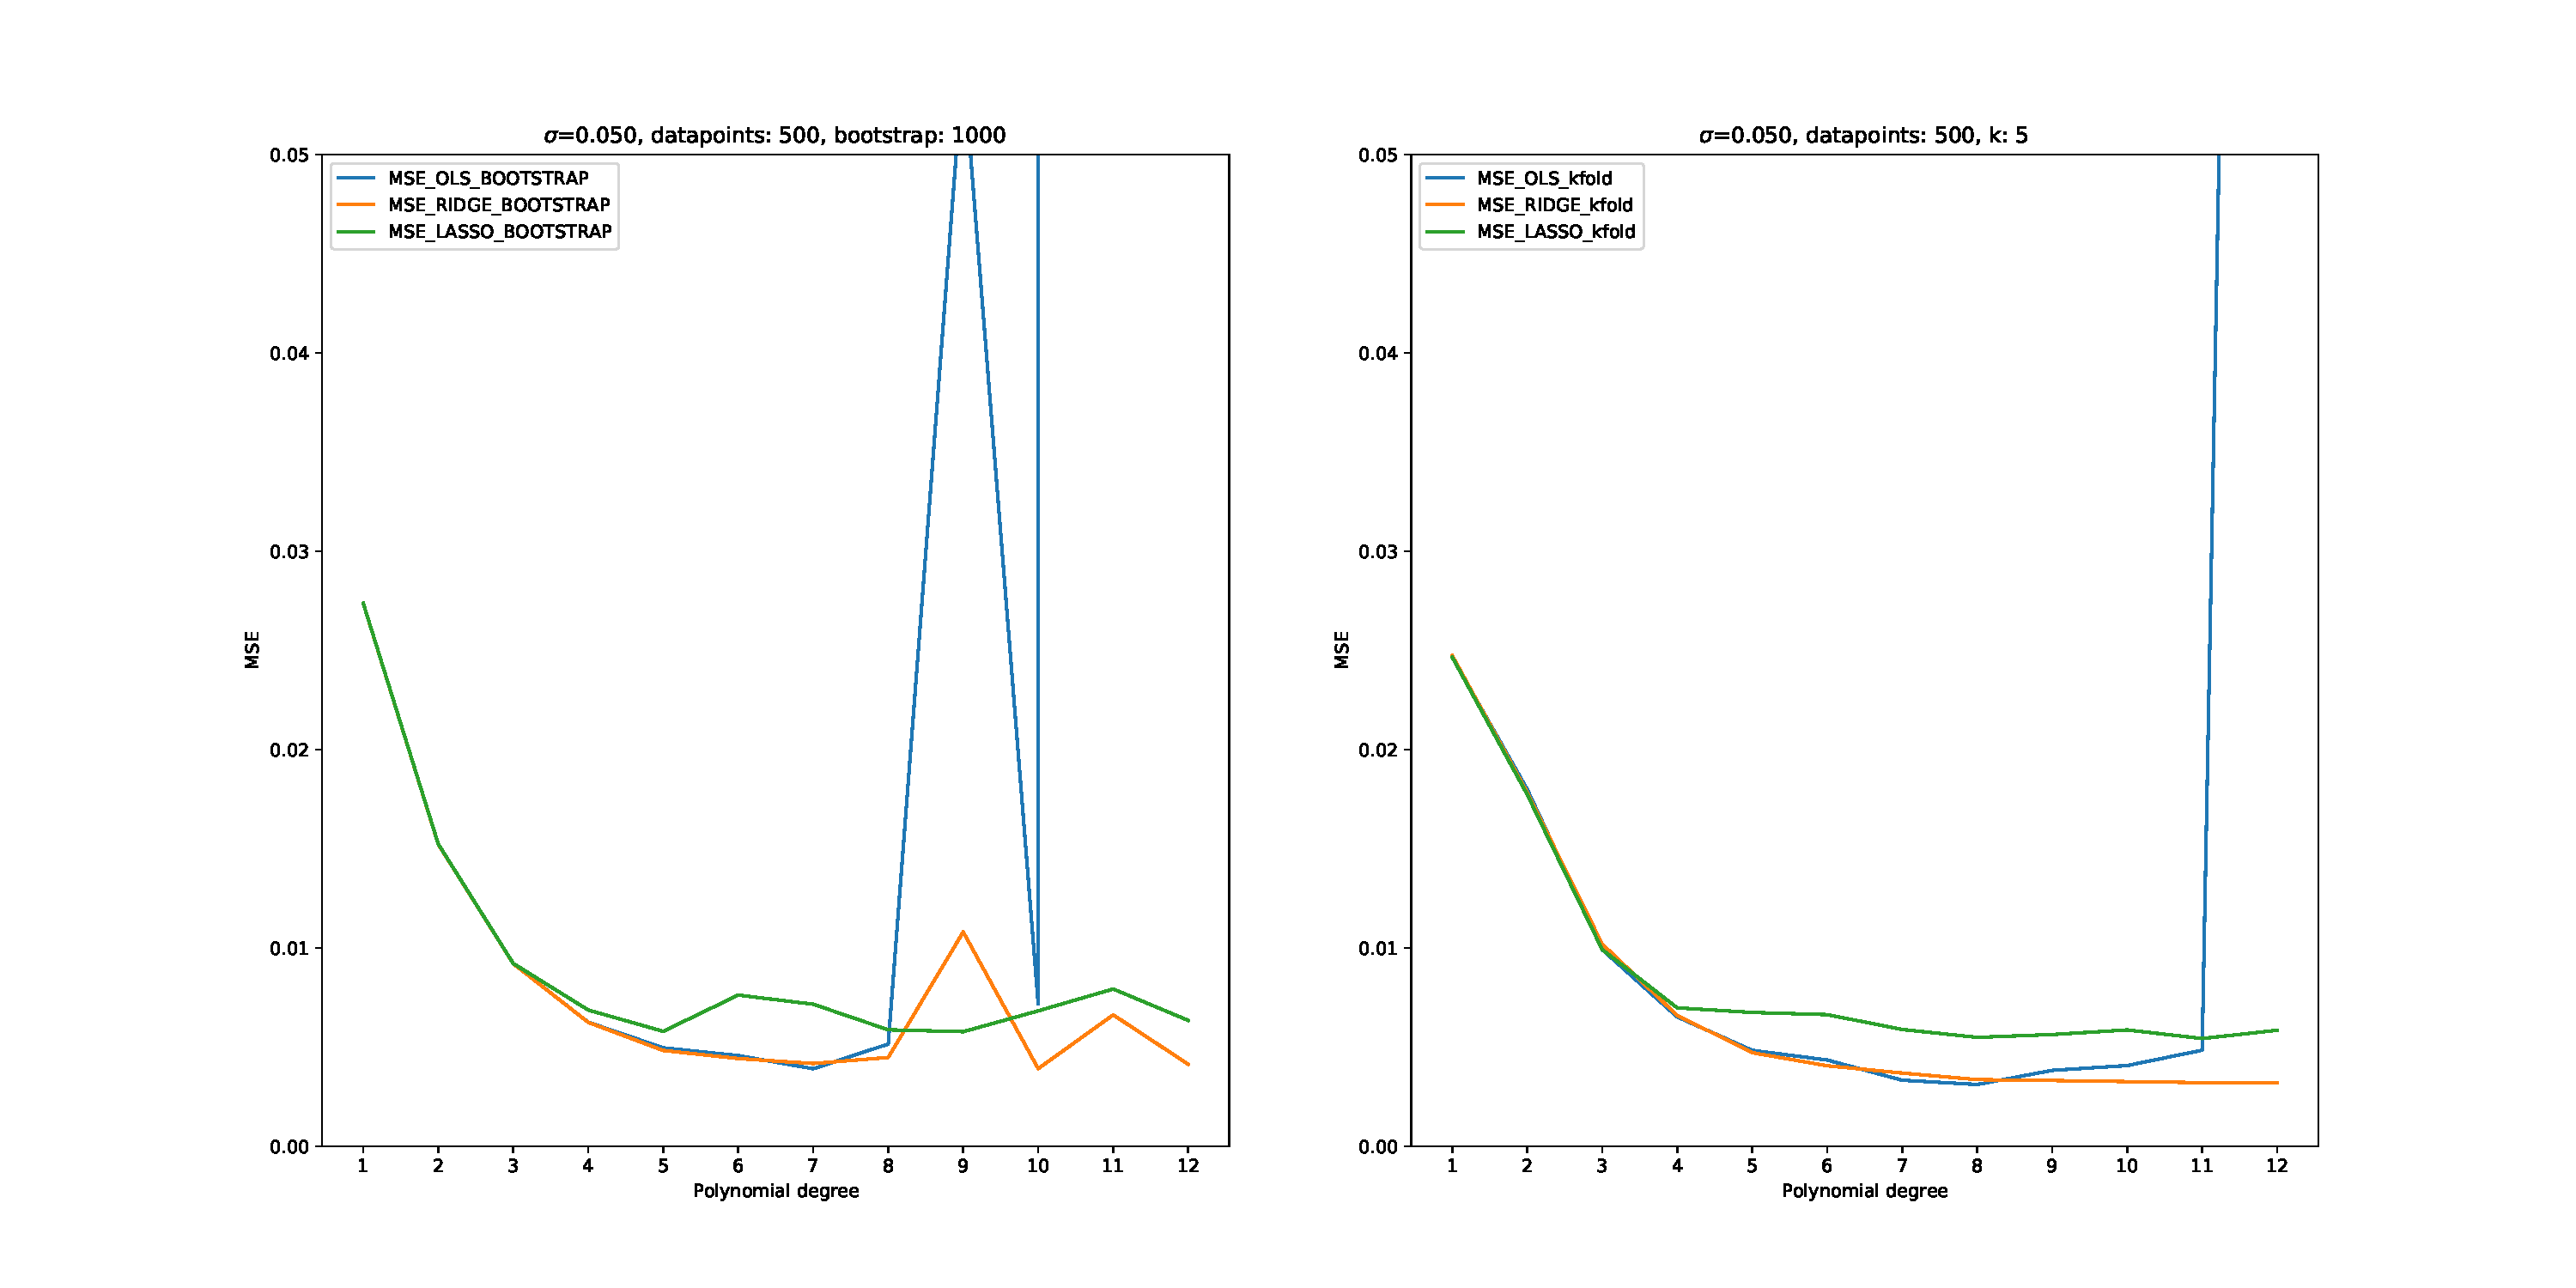
\includegraphics[width=0.95\textwidth]{MSE_different_methods_Franke.pdf}
\caption[Test MSE for LASSO, Rigde and OLS regression]{Test MSE for LASSO, Rigde and OLS regression. Estimated using Bootstrap (left) or k-Fold Cross validations. The exact parameters can be found in the graph's title.}
\label{fig:LASSO_Bias_Variance}
\end{figure}
\begin{figure}[H]
\centering
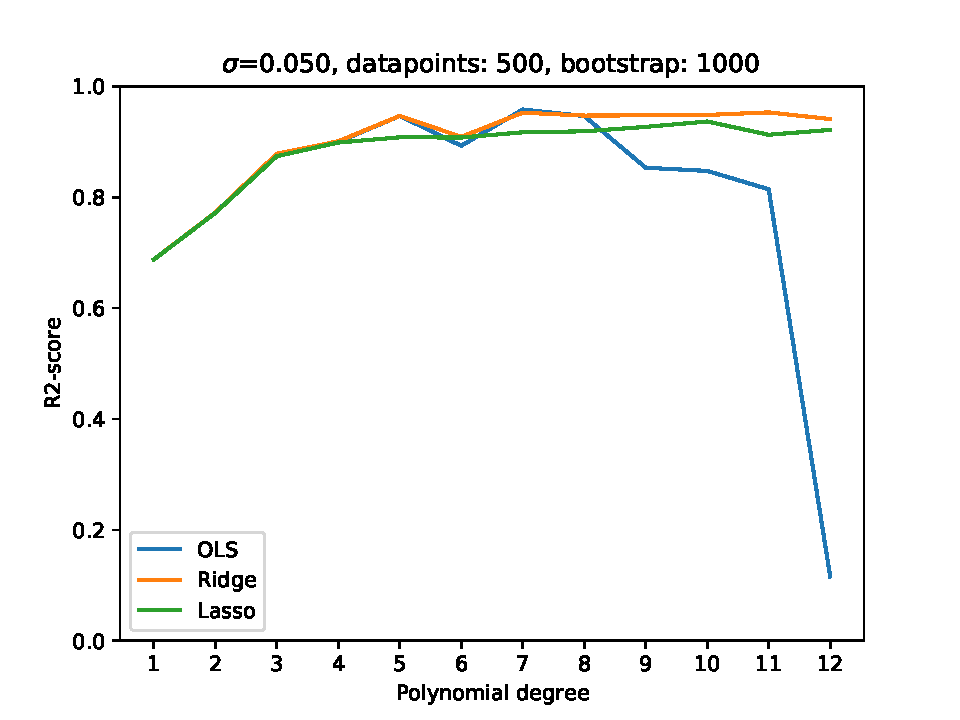
\includegraphics[width=0.95\textwidth]{R2_bootstrap_different_methods_Franke.pdf}
\caption[Test $R^2$-value for LASSO, Rigde and OLS regression]{Test $R^2$-value for LASSO, Rigde and OLS regression. Estimated using Bootstrap (left) or k-Fold Cross validations. The exact parameters can be found in the graph's title.}
\label{fig:LASSO_Bias_Variance}
\end{figure}

As expected from the theory, increasing the model complexity lead to a decreased Mean-Square-Error and an increased R2-Score for all three methods when fitting the Franke Function. However, as can be seen in figures XXX and XXX, the mean square error for the Ordinary Least Square approximation suddenly raises sharply (and the R2 score drops sharply) after some complexity is reached: This behaviour cannot be observed with LASSO and Ridge. Neither LASSO nor Ridge give conceivably better results than OLS when looking at the complexity giving the best results, that is, with the chosen parameters, OLS, LASSO and Ridge regression are about equally fast. As OLS is the most basic method, easiest to implement and also fastest, we figured out that it is the most suitable method for this problem - adding more complexity while avoiding a high variance (Ridge or LASSO) does not improve the quality of the fit.  Another interesting observation is that there is much more fluctuation in the MSE when using bootstrap than when using 5-fold Cross validation. We are not quite sure why this happens, but we assume that one possible cause is that when using bootstrap, some very "undesirable" combinations of values might be chosen, which leads to a very high Bootstrap. Thus, the graphs might look smoother when running more Bootstrap-samples. Another reason is that the training set in the Bootstrap method is not equally large as the training set when using 5-fold cross validation (75\% vs 80\%). We also observed that Bootstrap is more time-demanding than k-fold Cross Validation. The large deviation between LASSO and OLS is due to the aforementioned error.
\subsubsection{Map data}
\subsection{Bias-Variance tradeoff}

\subsubsection{Franke Function}
\begin{figure}[H]
\centering
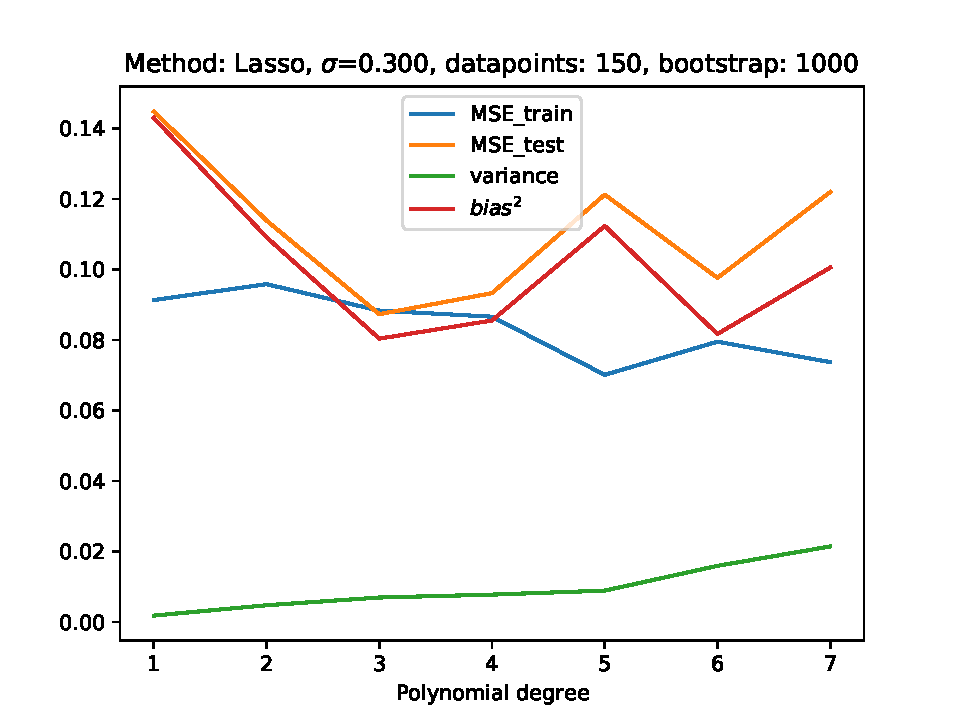
\includegraphics[width=0.65\textwidth]{Bias_Variance_LASSO.pdf}
\caption[Bias, Variance, MSE \& training MSE as a function of the polynomial degree using LASSO regression]{Bias, Variance, MSE \& training MSE as a function of the polynomial degree using LASSO regression. The values for $\sigma$, the size of the dataset and the number of bootstraps can be found in the title.}
\label{fig:LASSO_Bias_Variance}
\end{figure}
\begin{figure}[H]
\centering
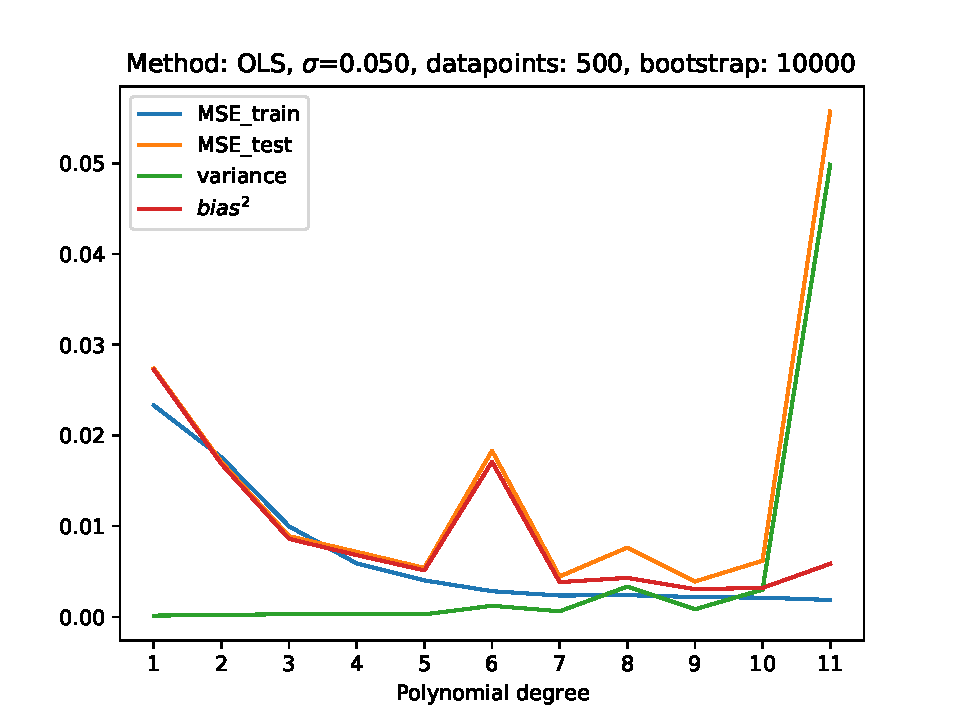
\includegraphics[width=0.65\textwidth]{Bias_Variance_OLS.pdf}
\caption[Bias, Variance, MSE \& training MSE as a function of the polynomial degree using OLS regression]{Bias, Variance, MSE \& training MSE as a function of the polynomial degree using OLS regression. The values for $\sigma$, the size of the dataset and the number of bootstraps can be found in the title.}
\label{fig:Bias_Variance}
\end{figure}
\begin{figure}[H]
\centering
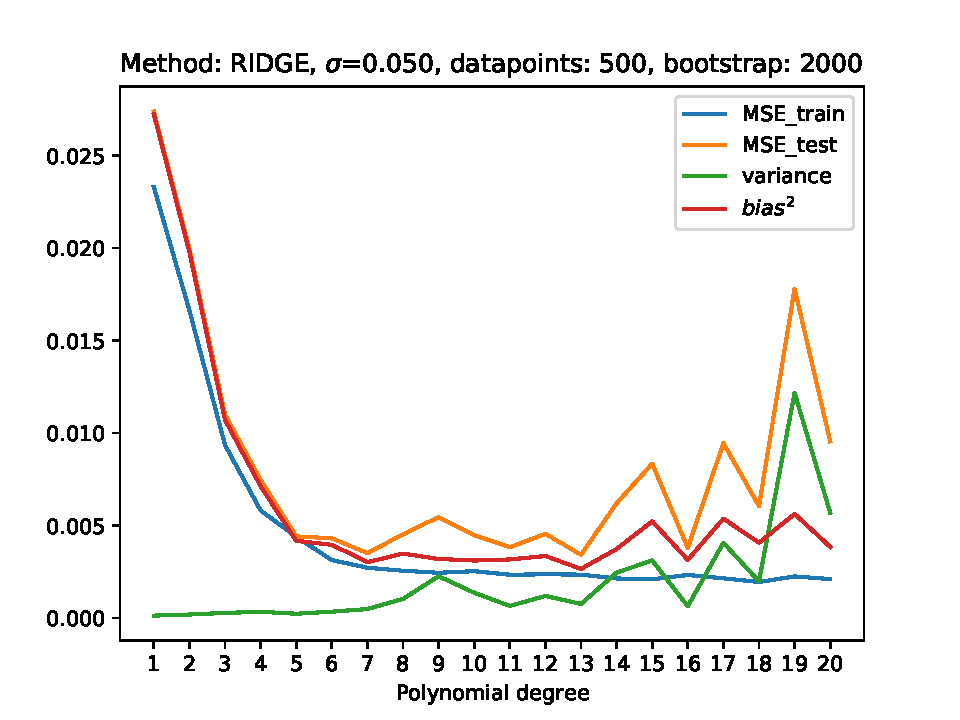
\includegraphics[width=0.65\textwidth]{Bias_Variance_RIDGE.pdf}
\caption[Bias, Variance, MSE \& training MSE as a function of the polynomial degree using Ridge regression]{Bias, Variance, MSE \& training MSE as a function of the polynomial degree using Ridge regression. The values for $\sigma$, the size of the dataset and the number of bootstraps can be found in the title.}
\label{fig:Ridge_Bias_Variance}
\end{figure}
Figures XXX, XXX and XXX show the MSE, the Training-MSE, the Variance, and the bias for the Franke Function. In all figures, the aforementioned statement that the variance increases and the bias decreases with increasing model complexity, hold true. Especially for the OLS, we see that this resembles  figure XXX on page XXX in HASTIE a lot. One can see that OLS is more prone to a higher variance at higher polynomial degrees, as is expected - shrinkage methods explicitly reduce the variance. There seems to be especially little variation in the LASSO approach, however, it is possible that this is due to the aforementioned issue with LASSO regression, as we have not found the ideal LASSO-coefficients due to the large error.
\subsubsection{Map data}

\section{Conclusion}
``I always thought something was fundamentally wrong with the universe'' \citep{hastie01statisticallearning}

\bibliographystyle{plain}
\bibliography{references}
\end{document}